\documentclass{scrreprt}
%\usepackage{float}
\usepackage{fullpage}
\usepackage{caption}
\usepackage{subcaption}
\usepackage{listings}
\usepackage{underscore}
\usepackage{tabularx}
\usepackage{longtable}
\usepackage{graphicx}
\usepackage[bookmarks=true]{hyperref}
\usepackage{pdfpages}
\usepackage{cite}

\setcounter{secnumdepth}{3}
\setcounter{tocdepth}{3}

\definecolor{airforceblue}{rgb}{0.66, .0, 0.36}

\hypersetup{
%    bookmarks=false,    % show bookmarks bar?
    pdftitle={Software Requirement Specification},    % title
    pdfauthor={Homer J. Simpson},                     % author
    pdfsubject={TeX and LaTeX},                        % subject of the document
    pdfkeywords={TeX, LaTeX, graphics, images}, % list of keywords
    colorlinks=true,       % false: boxed links; true: colored links
    linkcolor=blue,       % color of internal links
    citecolor=black,       % color of links to bibliography
    filecolor=black,        % color of file links
    urlcolor=purple,        % color of external links
    linktoc=page            % only page is linked
}

\def\myversion{1.0 }

\newcounter{myCounter}[subsubsection] 
\newcounter{mySubCounter}[myCounter] 

\makeatletter
\newcommand{\reqLabel}[1]{%
\myLabel{#1}{Req}}
\makeatother

\makeatletter
\newcommand{\reqLabelB}[1]{%
\myLabelB{#1}{Req}}
\makeatother

\makeatletter
\newcommand{\specLabel}[1]{%
\myLabel{#1}{Spec}}
\makeatother

\makeatletter
\newcommand{\specLabelB}[1]{%
\myLabelB{#1}{Spec}}
\makeatother

\makeatletter
\newcommand{\defLabel}[1]{%
\myLabel{#1}{Def}}
\makeatother

\makeatletter
\newcommand{\nfLabel}[1]{%
\myLabel{#1}{NF}}
\makeatother

\makeatletter
\newcommand{\rightMouse}{%
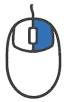
\includegraphics[width=15pt]{img/rightMouse.jpg}}
\makeatother

\makeatletter
\newcommand{\rightArrow}{%

\includegraphics[width=10pt]{img/rightArrow.png}\hspace{1mm}}
\makeatother

\makeatletter
\newcommand{\of}{%
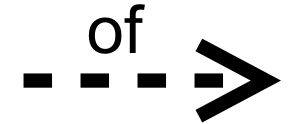
\includegraphics[height=8pt]{img/arrowOf.png}\hspace{1mm}}
\makeatother
\makeatletter
\newcommand{\extends}{%
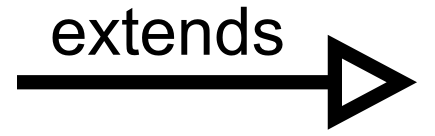
\includegraphics[height=8pt]{img/arrowExtends.png}\hspace{1mm}}
\makeatother
\makeatletter
\newcommand{\has}{%
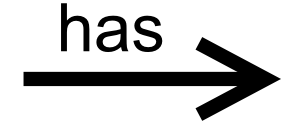
\includegraphics[height=8pt]{img/arrowHas.png}\hspace{1mm}}
\makeatother

%%%%%%%%%%%%%%%%%%%%%%%%%%%%%%%%%% Variante 1 %%%%%%%%%%%%%%%%%%%%%%%%%%%%%%%%%%%%%%%
\newcommand{\layerOne}[1]{\chapter{#1}}
\newcommand{\layerOneStar}[1]{\chapter*{#1}}
\newcommand{\layerTwo}[1]{\section{#1} \setcounter{myCounter}{0}}
\newcommand{\layerThree}[1]{\subsection{#1} \setcounter{myCounter}{0}}
\newcommand{\layerFour}[1]{\subsubsection{#1}}

\makeatletter
	\newcommand{\myLabel}[2]{%
		\refstepcounter{myCounter}
		\def\@currentlabel{#2-\thesubsubsection.\arabic{myCounter}}% Update label
		\raisebox{\f@size pt}\phantomsection
		\label{req:#1}
		\hspace{-\f@size pt}
		#2-\thesubsubsection.\arabic{myCounter}}
\makeatother

%\makeatletter
%	\newcommand{\myLabelFour}[2]{%
%		\refstepcounter{myCounter}
%		\def\@currentlabel{#2-\thesubsection.\arabic{myCounter}}% Update label
%		\raisebox{\f@size pt}\phantomsection
%		\label{req:#1}
%		#2-\thesubsection.\arabic{myCounter}}
%\makeatother

\newcommand{\kmh}{$kmh^{-1}$}

\makeatletter
	\newcommand{\myLabelB}[2]{%
		\refstepcounter{mySubCounter}
		\def\@currentlabel{#2-\thesubsubsection.\arabic{myCounter}\alph{mySubCounter}}%
		% Update label
		\raisebox{\f@size pt}\phantomsection
		\label{req:#1}
		\hspace{-\f@size pt}
		#2-\thesubsubsection.\arabic{myCounter}\alph{mySubCounter}}
\makeatother

%%%%%%%%%%%%%%%%%%%%%%%%%%%%%%%%%% Variante 2 %%%%%%%%%%%%%%%%%%%%%%%%%%%%%%%%%%%%%%%
%
%\newcommand{\layerOne}[1]{\part{#1}}
%\newcommand{\layerOneStar}[1]{\part*{#1}}
%\newcommand{\layerTwo}[1]{\chapter{#1}}
%\newcommand{\layerThree}[1]{\section{#1}}
%
%\makeatletter
%	\newcommand{\myLabel}[2]{%
%		\refstepcounter{myCounter}
%		\def\@currentlabel{#2-\thesubsection.\arabic{myCounter}}% Update label
%		\raisebox{\f@size pt}\phantomsection
%		\label{req:#1}
%		#2-\thesubsection.\arabic{myCounter}}
%\makeatother
%
%\makeatletter
%	\newcommand{\myLabelB}[2]{%
%		\refstepcounter{mySubCounter}
%		\def\@currentlabel{#2-\thesubsection.\arabic{myCounter}\alph{mySubCounter}}% Update label
%		\raisebox{\f@size pt}\phantomsection
%		\label{req:#1}
%		#2-\thesubsection.\arabic{myCounter}\alph{mySubCounter}}
%\makeatother
%
%%%%%%%%%%%%%%%%%%%%%%%%%%%%%%%%%% Variante Ende %%%%%%%%%%%%%%%%%%%%%%%%%%%%%%%%%%%%%%%

\makeatletter
  \newcommand{\myRef}[1]{
  \ref{req:#1}}
\makeatother

\makeatletter
  \newcommand{\lowItem}{
  \vspace{-2.5mm}\item}
\makeatother

\makeatletter
  \newcommand{\comment}{
  \hspace{1em} \textit{Comment}}
\makeatother

\makeatletter
  \newcommand{\issue}[1]{
  \href{https://github.com/xmf-xmodeler/Mosaic/issues/#1}{Git Issue \##1}}
\makeatother
\title{
\flushright
\rule{15.5cm}{5pt}\vskip1cm
\Huge{SOFTWARE REQUIREMENTS\\ SPECIFICATION}\\
\vspace{2cm}
for\\
\vspace{2cm}
XModeler\\
\vspace{2cm}
\LARGE{Release 1.0\\}
\vspace{2cm}
\LARGE{Version \myversion approved\\}
\vfill
\rule{15.5cm}{5pt}
}
\date{}
\usepackage{hyperref}
\begin{document}
\maketitle
%\includepdf[pages=1]{img/title.pdf}
\newpage
\phantomsection
\addcontentsline{toc}{chapter}{Contents}

\tableofcontents

\clearpage
\phantomsection
\addcontentsline{toc}{chapter}{Revision History}
\layerOneStar{Revision History}

\layerOne{Requirements} 

\begin{tabularx}{\textwidth}[t]{|l|X|} \hline
\reqLabel{general:r1} & Some requirements may be optional. \myRef{general:s1}\\ \hline
\end{tabularx}

\layerTwo{Web Site} 

\begin{tabularx}{\textwidth}[t]{|l|X|} \hline
\reqLabel{Website:General:r1} & 
The website is available online. \\\hline& 
A slightly different version is available in XModeler. \\\hline OR & The online version is accessed from XModeler, but unavailable when offline. \\\hline OR& XModeler tries to access the online version, but keeps a offline version as backup. \\\hline &
The online version cannot use the XModeler's hijacking mode for references.\\
\hline
\reqLabel{Website:General:r2} & 
The website will have several parts: 
The online home page, 
the in-tool home page, 
online content, 
in-tool content,
online content which is available offline.
In-tool content can access online content. Online content cannot access in-tool content. \\
\hline
\end{tabularx}

\layerThree{Content} 

\begin{tabularx}{\textwidth}[t]{|l|X|} \hline
\reqLabel{Website:Content:r0} & 

\begin{itemize}
\lowItem XModeler
\begin{itemize}
  \lowItem What is XModeler?
	\lowItem Getting started
	\begin{itemize}
		\lowItem Install guide
		\lowItem Tutorial
	\end{itemize}
	\lowItem Help
	\begin{itemize}
		\lowItem API
		\lowItem Language concepts
		\lowItem Snippets $^X$
		\lowItem Bluebook $^X$
	\end{itemize}
\end{itemize}
\lowItem Literature
\begin{itemize}
	\lowItem Articles, Papers
		\begin{itemize}
		\lowItem Our Articles, Papers
		\lowItem Conferences
		\lowItem List of others' literature
	\end{itemize}
	\lowItem Lecture Slides and other material for students $^O$
\end{itemize}
\lowItem External Links
\begin{itemize}
	\lowItem git
	\lowItem shu
	\lowItem ude
\end{itemize}
\lowItem Contact
\begin{itemize}
	\lowItem Who are we
	\lowItem How to contact us
	\lowItem Impressum
\end{itemize}
\end{itemize}
 $^X$: Not available online\newline
 $^O$: Only available online\newline
\newline
Is any material we use copyrighted? Are icons and logos in XModeler our work? If they are from any "`free"' source, are there any conditions on them?\newline
Do we need any legal advice? Disclaimers?
\\
%\vspace{-15mm}\\
\hline
\reqLabel{Website:Content:r1} & 
The website should include a install guide\\
\hline
\reqLabelB{Website:Content:r1a} & 
The install guide should be split into several parts, after each (and before first) some checks to see if step worked. \\
\hline
\reqLabelB{Website:Content:r1b} & 
The install guide should contain common problems. \\
\hline
\reqLabel{Website:Content:r10} & 
The website should include a tutorial.\\
\hline
\reqLabel{Website:Content:r2} & 
The website should include a "`API"', explaining the basic data types and classes.\\
\hline
\reqLabel{Website:Content:r3} & 
The website should include an explanation of basic language concepts. (grammar, operators)\\
\hline
\reqLabel{Website:Content:r4} & 
The website should include snippets. (Small examples on a specific topic, like how to read from a file)\\
\hline
\reqLabel{Website:Content:r5} & 
The website should include a list of literature, with links if possible.\\
\hline
\reqLabel{Website:Content:r6} & 
The website should include a link to git, Maybe direct links to the Issues?\\
\hline
\reqLabel{Website:Content:r7} & 
The website should include information about contact. \textit{Whom was it made by? How do I contact them, report a bug?\ldots}\\
\hline
\end{tabularx}

\layerThree{Design} 
\begin{tabularx}{\textwidth}[t]{|l|X|} \hline
\reqLabel{Website:Design:r1} & 
The design should have a primary and a secondary colour. These, together with gray-scale colours should be used predominantly. 
\myRef{Website:Design:s1}, \myRef{Website:Design:s2}\\
\hline
\reqLabel{Website:Design:r2} & The website is split vertically: Title, Links, local Links, Content
\\\hline
\end{tabularx}

\newpage
\layerTwo{Changes on Intrinsics}

\begin{tabularx}{\textwidth}[t]{|l|X|} \hline
\reqLabel{MultilevelIntrinsicEditing:General:r1} & 
The user may want the changes to affect all existing instances.\\\hline
\reqLabel{MultilevelIntrinsicEditing:General:r2} & 
The user may want the changes to affect all future instances.\\\hline
\reqLabel{MultilevelIntrinsicEditing:General:r3} & 
The user may want any alerts to be suppressed until he finishes his changes.\\\hline
%\reqLabel{MultilevelIntrinsicEditing:General:q1} & 
%How do we find all usages?\\\hline
\end{tabularx}

\layerThree{Add}

\begin{tabularx}{\textwidth}[t]{|l|X|} \hline
\reqLabel{MultilevelIntrinsicEditing:Add:r1} & 
\textbf{The user adds a new intrinsic attribute.} Every instance on the appropriate level should get a slot for the Attribute. No slot will be provided before the given level is reached. \textsl{Isn't there a constraint that an element must have all slots for which the of() has an attribute?} Unless a default value is given, all instances have to be supplied with new data.
\\&\multicolumn{1}{c|}{\includegraphics[width=200pt]{img/intrinsics/IntrinsicAdd.pdf}}
\\\hline
\reqLabel{MultilevelIntrinsicEditing:Add:r2a} & 
\textbf{The user adds a new intrinsic attribute causing a name clash on lower levels.} This means that an attribute on a lower level would --- intended or not --- override or hide the newly created attribute.
\\&\multicolumn{1}{c|}{\includegraphics[width=200pt]{img/intrinsics/IntrinsicAddClashLower.pdf}}
\\\hline
\reqLabel{MultilevelIntrinsicEditing:Add:r2b} & 
\textbf{The user adds a new intrinsic attribute causing a name clash on higher levels.} Basically the same possible conflicts as above, but a higher degree of intention can be assumed.\\\hline
%\reqLabel{MultilevelIntrinsicEditing:Add:r4} & 
%\\
%\hline
\end{tabularx}

\layerThree{Delete}

\begin{tabularx}{\textwidth}[t]{|l|X|} \hline
\reqLabel{MultilevelIntrinsicEditing:Delete:r1} & 
\textbf{The user deletes an intrinsic attribute.} All usages should be removed as well. Otherwise they would lose their connection to their original definition.
\\&\multicolumn{1}{c|}{\includegraphics[width=200pt]{img/intrinsics/IntrinsicRemove.pdf}}
\\\hline
%\reqLabel{MultilevelIntrinsicEditing:Delete:r2} & 
%\\\hline
%\reqLabel{MultilevelIntrinsicEditing:Delete:r3} & 
%\\
%\hline
\end{tabularx}

\layerThree{Change Level of Attribute}

\begin{tabularx}{\textwidth}[t]{|l|X|} \hline
\reqLabel{MultilevelIntrinsicEditing:Add:r3} & 
T\textbf{he user adds a new intrinsic attribute intentionally causing a name clash on lower levels}, therefore raising the level of the attribute. The intrinsic attributes in the lower classes must be removed. Opposite of \myRef{MultilevelIntrinsicEditing:ChangeA:r1}
\\&\multicolumn{1}{c|}{\includegraphics[width=350pt]{img/intrinsics/IntrinsicRaise.pdf}}
\\\hline
\reqLabel{MultilevelIntrinsicEditing:ChangeA:r1} & 
\textbf{The user deletes an intrinsic attribute in a class and adds it to all that class' instances}. Opposite of 
\myRef{MultilevelIntrinsicEditing:Add:r3}. Would mean adding redundancy and is therefore unlikely to happen.\\\hline
\reqLabel{MultilevelIntrinsicEditing:ChangeA:r2} & 
\textbf{The user renames an existing attribute.} In addition to the potential problems of adding one attribute and deleting another one, this case is different as the attribute should remain unchanged apart from it's name. This makes this scenario a genuine one, that means it is not a combination of other scenarios.
\\&\multicolumn{1}{c|}{\includegraphics[width=200pt]{img/intrinsics/IntrinsicRename.pdf}}
\\\hline
%\reqLabel{MultilevelIntrinsicEditing:ChangeA:r3} & 
%\\\hline
%\reqLabel{MultilevelIntrinsicEditing:ChangeA:r4} & 
%\\
%\hline
\end{tabularx}

\layerThree{Change Level Of Class}

\begin{tabularx}{\textwidth}[t]{|l|X|} \hline
\reqLabel{MultilevelIntrinsicEditing:ChangeC:r1} & 
The user changes the level of a class: All instances have to be of lower level than the class. All intrinsic attributes have to be of lower level than the class. All classes above the class must comply or be changed as well. No gap must be left between levels.  \\\hline
%\reqLabel{MultilevelIntrinsicEditing:ChangeC:r2} & 
%\\\hline
\end{tabularx}
\newpage

\layerThree{Checks}

%An object with isIntrinsic=false has no Attributes with isIntrinsic=true\\
\begin{itemize}
	\item An Attribute, which is intrinsic, can only be in (or added to) Objects, which are intrinsic and are of Class.
	\item An Attribute, which is not intrinsic, can only be in (or added to) Objects, which are of Class.
	\item \textit{An Object with isIntrinsic=false has no Attributes with isIntrinsic=true}
	\item \textit{An Object which is not of Class has no Attributes}
	
	\item An Object which is intrinsic on level 2 or more must extend Class/MetaClass
	\item An Object which is intrinsic on level 1 must be of a something extending Class/MetaClass but must not extend Class/MetaClass
	\item An Object which is intrinsic on level 0 must neither be of a something extending Class/MetaClass nor extend Class/MetaClass
	
	\item The level of an Object that is intrinsic must be 1 less the of's level, unless the of is not intrinsic.
	
	\item An Attribute, which is not intrinsic, of an Object, which is of Class (implied by a previous check), must have a slot at all instances.
	\item \textit{All instances of an Object, which is of Class (implied by a previous check), must have a slot for every of's non-intrinsic Attribute.}
	
	\item An Attribute, which is intrinsic, of an Object, which is of Class, must have a slot at all instances (or instances' instances...) which are on the given level.
\end{itemize}
 
\layerThree{Addons-Essen Existing Implementation}

\layerFour{MetaAdaptor new()}
\begin{itemize}
	\item 1: A class with isIntrinsic=false creates an instance, where isIntrinsic is false as well. Normal behaviour.
	\item 2: A class with isIntrinsic=false creates an instance, where isIntrinsic is true. The instance needs a level, which has to be provided in some way. This class must extend Class/MetaClass to be on levels 2 or higher
	\item 3: A class with isIntrinsic=true creates an instance, the level is decreased. If the class is higher than level 2(=the instance is at least at level 2) it must extend Class/MetaClass
\end{itemize}

If case 2 would provide the level by argument, then the function would be callable on level-aware objects as well. \textit{An object of level 3 instantiating to level 5?} The newToLevel must check and throw an error in this case. Alternatively it could be unavailable by splitting classes which would be a lot of extra work and would eventually resulting in throwing an error anyway...

\textbf{MetaAdaptor} is of \textbf{Class}. Shouldn't it be Adapt\textbf{e}r?

\begin{verbatim}
=  @Operation new():Object
\end{verbatim}
o is created by the Kernel function instead of super class Class' new(). To prevent the creation of slots, Class' new() function is copied and modified (+,-,=)\\
A are all Attributes, intrinsicA is an empty set
\begin{verbatim}
=      let o = Kernel_mkObj();
=          A = self.allAttributes();
+         intrinsicA = Set{}
\end{verbatim}
The of link is set.\\
A loop, aimed at emptying A (all Attributes) is started
\begin{verbatim}
=     in Kernel_setOf(o,self);
=        @While not A->isEmpty do
=          let a = A->sel
\end{verbatim}
for each attribute: if it is intrinsic, and the level too low, then it is meant to be skipped in creating slots. It is put in the set "`intrinsicA"'. \textbf{For a new unified constructor we can assume that no attribute is intrisic on non-intrinsics classes, so the exclusion does nothing, leaving the new set empty.}
\begin{verbatim}
+          in if a.isIntrinsic and a.instLevel < o.of().level - 1
+             then
+               intrinsicA := intrinsicA.including(a)
+             else
\end{verbatim}
Otherwise, if the Attribute is to be instantiated. Then it is added, if available by the init function, as Class would do\\
In both cases it is removed from the list A.
\begin{verbatim}
=                if a.init <> null
=               then
=                 Kernel_addAtt(o,a.name,a.init.invoke(o,Seq{}))
=               else
=                 Kernel_addAtt(o,a.name,a.type.default())
+               end
=             end;
=             A := A->excluding(a)
=          end
=        end;
\end{verbatim}
Now, the attributes are done. The parents are set. If it does not inherit form Classifier it returns false? 
It originally returned o instead. \textbf{Both seem to be pointless, so the else should be dropped altogether.} After that the object/class is being initialized. 
\begin{verbatim}
=        if self.inheritsFrom(Classifier)
=        then
=          o.parents := o.defaultParents()
=        else
+          false
-          o
=        end;
=        o.init();
\end{verbatim}
The following part is used for case 2, creating a level-aware class form a level-agnostic, and for case 3, reducing the level on level-aware classes. Case 1 would simply finish here (except for two {\ttfamily end}s). \textbf{For a new unified constructor, case 2 would not go through a no-argument function. Therefor a new function is needed.}
It checks if of() is MetaAdaptor, in which case a dialogue will open and ask for a level. MetaClass will then be a parent. This should imply a level of at least 2, which is not checked here.\\
The level input by dialogue must be removed. A {\ttfamily newToLevel(level:Integer)} should be the replacement for these cases.
\begin{verbatim}
+        if self.of() = Extensions::MetaAdaptor
+        then
+          o.level := xmf.getInteger("Metaebene","Auf welcher Metaebene soll 
+					sich diese Entität befinden?",3);
+           o.addParent(FMML::MetaClass)
+         else
\end{verbatim}
Otherwise (if of() is not MetaAdaptor) this is an instance of a level-aware class. If the level is more than 2 then the instance's level must be at least 2, implying it is a MetaClass. Then the instance's level is set to the next lower level. Unless a special case (Why?) requires it to be 2.\\
If the level was less than 2. It is just decreased by one. Only level 1 and 2 should enter this path, resulting in level 1 or 0. Level 0 cannot access this function, as this is meant to be prevented elsewhere. Therefore levels lower than 0 cannot occur if prevented properly.
\begin{verbatim}
+           if o.of().level > 2
+           then
+             o.addParent(FMML::MetaClass);
+             if o.of().of().allAttributes()->exists(a |
+               a.name = "level".asSymbol())
+             then
+               o.level := o.of().level - 1
+             else
+               o.level := 2
+             end
+           else
+             o.level := o.of().level - 1
+           end
+         end;
\end{verbatim}
The skipped intrinsic attributes are added (as Attributes) to the instance. As no intrinsics should remain on level 0, o's level must be at least 1.
\begin{verbatim}
+         @While not intrinsicA.isEmpty() do
+           let intA = intrinsicA.sel()
+           in o.add(intA);
+              intrinsicA := intrinsicA.excluding(intA)
+           end
+         end;
+?         if Root.contents.keys().includes("TargetPackage".asSymbol())
+?         then
+?           TargetPackage.add(o)
+?         else
+?           false
+?         end;
+?         o
=      end
=    end
\end{verbatim}

\layerFour{newToLevel}

\begin{verbatim}
  @Operation newToLevel(level:integer):Object
\end{verbatim}
\begin{verbatim}
      let o = Kernel_mkObj();
          A = self.allAttributes();
     in Kernel_setOf(o,self);
        @While not A->isEmpty do
          let a = A->sel
             if a.init <> null
             then
               Kernel_addAtt(o,a.name,a.init.invoke(o,Seq{}))
             else
               Kernel_addAtt(o,a.name,a.type.default())
             end;
             A := A->excluding(a)
          end
        end;
        if self.inheritsFrom(Classifier)
        then
          o.parents := o.defaultParents()
        end;
        o.init();
\end{verbatim}
Now case 2 is done
\begin{verbatim}
        if self.of() = Extensions::MetaAdaptor
        then
           o.level := level;
           o.Isintrinsic = true;
           o.addParent(FMML::MetaClass)
         end;
				
         if Root.contents.keys().includes("TargetPackage".asSymbol())
         then
           TargetPackage.add(o)
         else
           false
         end;
         o
      end
    end
\end{verbatim}

%Intrinsics are copied (or linked) through the levels. So allAttributes returns the skipped attributes because the are stored in that level. \\
Another approach would not copy them through the levels. Instead the allAttributes function would check all higher levels for skipped attributes.

\layerThree{Multiplicity}

\begin{verbatim}
context Attribute
  @Operation setMult(mult)
    if mult.isKindOf(String)
    then self.setMultString(mult)
    else self.setProperty("mult",mult)
    end
  end
\end{verbatim}
If multiplicity is a string, is needs to be parsed. Otherwise (what? int?) it is stored in "`mult"'.
\begin{verbatim}
context Attribute
  @Operation setMultString(multString:String)
    if self.mult().multString() <> multString
    then 
      self.setMult(self.decodeMultString(multString));
      self.updateTypeFromMult()
    end
  end
\end{verbatim}
mult() therefore returns something having a multString, which can be checked for changes. I it is changed it is decoded and then used in the original function, obviously returning a non-String type.
\begin{verbatim}
context Attribute
  @Operation decodeMultString(multString:String)
    try
      if multString = "" or multString = "1" or multString = null
      then Multiplicities::SingleMult(false)
      elseif multString = "!"
      then Multiplicities::SingleMult(true)
      else
        if multString = "*"
        then Multiplicities::CollectionMult(false,false,0,0)
        elseif multString = "$" or multString = "$*" 
        then Multiplicities::CollectionMult(true,false,0,0)
        else
          let ordered = multString.hasPrefix("$") then         //$
              rangeSeq = if ordered
                         then multString.subString(1,multString.size()).splitBy(".",0,0)
                         else multString.splitBy(".",0,0)
                         end then
              lowerBound = rangeSeq->head->asInt;
              hasUpperBound = not (rangeSeq->at(2) = "*") then
              upperBound = if hasUpperBound then rangeSeq->at(2)->asInt else 0 end
          in
            if hasUpperBound andthen upperBound < lowerBound
            then throw Exception("Invalid multiplicity '"+multString.toString() + "': upper bound is less than lower bound")
            else Multiplicities::CollectionMult(ordered,hasUpperBound,lowerBound,upperBound)
            end
          end
        end
      end
    catch(exception)
      throw Exception("Invalid multiplicity '"+multString.toString() + "'")
    end    
  end
\end{verbatim}
Multiplicities are a type, an abstract one. There is SingleMult and CollectionMult.
SingleMult only holds a boolean "`mandatory"' for $0..1$ and $1..1$
CollectionMult holds a lower, an upper bound, a boolean switching off the upper bound, and a boolean for making the order significant.

Is that separation neccessary? Isn't a SingleMult just a special case of CollectionMult. I saves storage to use a shorter one for standard cases.
Upper bound boolean would not be necessary if Integer has a Positive-Infinity-Value.

\newpage

\layerTwo{MeMo-Language}

\begin{tabularx}{\textwidth}[t]{|l|X|} \hline
\reqLabel{MeMo:General:r1} & 
The MultiLevel language MeMo requires\ldots\\
\hline
\reqLabel{MeMo:General:r2} & 
The MultiLevel language MeMo requires\ldots\\
\hline
\reqLabel{MeMo:General:r3} & 
The MultiLevel language MeMo requires\ldots\\
\hline
\end{tabularx}

\layerTwo{Kernel}
\layerTwo{X-Modeler}

\layerThree{Diagrams}

\layerFour{Multi-Level Diagram}

\layerThree{Forms}

\layerFour{FormsClient}

\begin{tabularx}{\textwidth}[t]{|l|X|} \hline
\reqLabel{Forms:FormsClient:r1} & 
The FormsClient receives messages to add components.\\
\hline
\reqLabel{Forms:FormsClient:r2} & 
The FormsClient must be able to display these components:
\begin{itemize}
  \item Label
  \item Textfield
  \item Textarea
  \item Checkbox
\end{itemize}
The component is determined by the type of the value.\\
\hline
\reqLabelB{Forms:FormsClient:r2a} & 
A boolean is shown as a Checkbox\\\hline
\reqLabelB{Forms:FormsClient:r2b} & 
An enum is shown as a drop-down-list\\\hline
\reqLabelB{Forms:FormsClient:r2c} & 
A short(?define) Strings or a number is shown as Textfield\\\hline
\reqLabelB{Forms:FormsClient:r2d} & 
A long(?define) String is shown as Textarea\\\hline
\reqLabel{Forms:FormsClient:r3} & 
Labels can be grouped with other components to form a key-value-pair.\\
\hline
\reqLabel{Forms:FormsClient:r4} & 
A form client has a listener for changes which will be transferred instantly to
the underlying model. There are no Save, Cancel or Undo buttons.\\\hline
\reqLabel{Forms:FormsClient:r5} & 
The FormsClient is linked to the underlying model.\\\hline
\reqLabel{Forms:FormsClient:r6} & 
The FormsClient's components are linked to the underlying model's parts
by an id.\\\hline
\comment & Labels should not be empty. \issue{34}\\\hline
\comment & Double click should not freeze the form. \issue{33}\\\hline
\end{tabularx}

\layerOne{Specifications} 

\setcounter{myCounter}{0}
\begin{tabularx}{\textwidth}[t]{|l|X|} \hline
\specLabel{general:s1} & Some specifications may be optional.
\myRef{general:r1}\\
\hline
\end{tabularx}

\layerTwo{Web Site}

\layerThree{Design} 
\begin{tabularx}{\textwidth}[t]{|l|X|} \hline
\specLabel{Website:Design:s1} & 
The design's primary colour is \#1155BB. \myRef{Website:Design:r1}\\
\hline
\specLabel{Website:Design:s2} & 
The design's secondary colour is \#22AA44. \myRef{Website:Design:r1}\\
\hline
\end{tabularx}

\layerTwo{XMF-Language}
\layerTwo{Kernel}
\layerTwo{X-Modeler}

\layerThree{Diagrams}

\layerFour{Multi-Level Diagram}

%\layerThree{Signals}
%
%\begin{tabularx}{\textwidth}[t]{|l|X|}
%	  \hline
%    \specLabel{signal:hp0} & Hp0: Stop aspect. One or two red lights. See
    % Fig.~\ref{fig:hp012}, \myRef{signal:1}, \myRef{signal:1a} \\	\hline
%		\specLabel{signal:hp1} & Hp1: Proceed aspect. One green light. See
		% Fig.~\ref{fig:hp012}, \myRef{signal:1}\\ \hline
%		\specLabel{signal:hp2} & Hp2: Slow aspect. One green over one yellow light.
		% Shown for speeds up to $60kmh^{-1}$. If no speed is specified by Zs3 the limit is $40kmh^{-1}$.
%		This default speed limit may be changed to $50kmh^{-1}$ or $60kmh^{-1}$. 
%		See Fig.~\ref{fig:hp012} \\ \hline
%\end{tabularx}
%
%\vspace{.5cm}
%\begin{figure}[ht!]
%	\centering
%	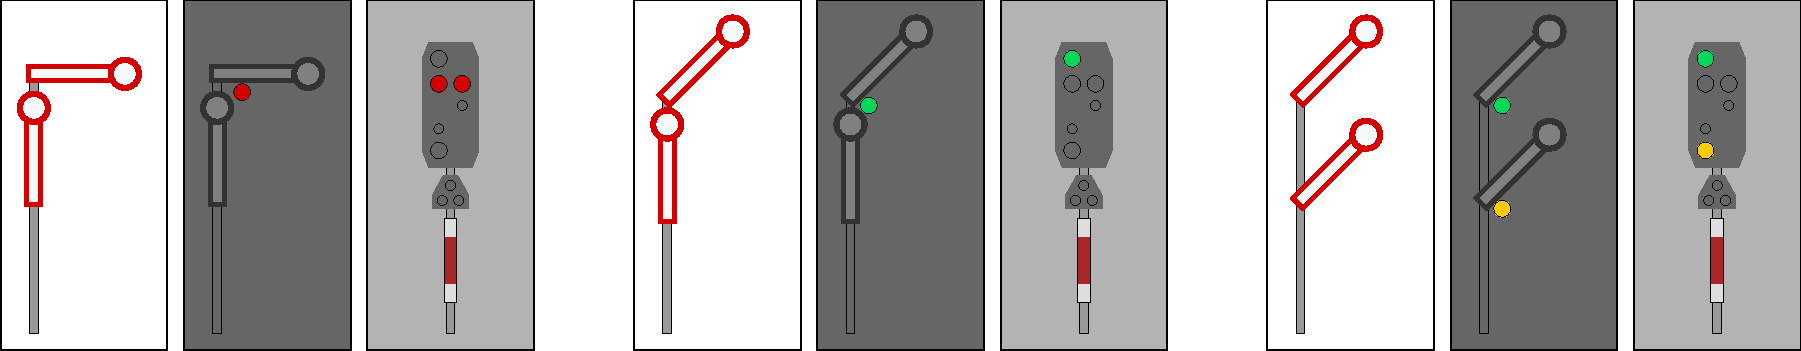
\includegraphics[width=420pt]{img/hp012.pdf}
%	\caption{from left to right: Hp0, Hp1, Hp2}
%	\label{fig:hp012}
%\end{figure} 

%\noindent

\layerOne{Other}

\layerTwo{git}

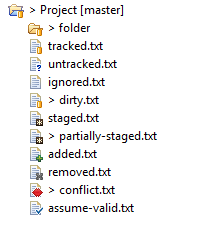
\includegraphics[width=120pt]{img/git-IconDecorations.png} %% von http://wiki.eclipse.org/EGit/User_Guide

\begin{itemize}
  \item \textbf{dirty (folder)} - At least one file below the folder is dirty; that
  means that it has changes in the working tree that are neither in the index nor in the repository.
  \item \textbf{tracked} - The resource is known to the Git repository and hence
  under version control.
  \item \textbf{untracked} - The resource is not known to the Git repository
  and will not be version controlled until it is explicitly added.
  \item \textbf{ignored} - The resource is ignored by the Git team provider. The
  preference settings under Team $>$ Ignored Resources, "derived" flag and
  settings from .gitignore files are taken into account.
  \item \textbf{dirty} - The resource has changes in the working tree that are
  neither in the index nor in the repository.
  \item \textbf{staged} - The resource has changes which have been added to the
  index. Note that adding changes to the index is currently possible only in the commit dialog via the context menu of a resource.
  \item \textbf{partially-staged} - The resource has changes which are added to the
  index and additional changes in the working tree that neither reached the index nor have been committed to the repository. See partial staging from the Git Staging view for how to do that.
  \item \textbf{added} - The resource has not yet reached any commit in the
  repository but has been freshly added to the Git repository in order to be tracked in future.
  \item \textbf{removed} - The resource is staged for removal from the Git
  repository.
  \item \textbf{conflict} - A merge conflict exists for the file.
  \item \textbf{assume-valid} - The resource has the "assume unchanged" flag. This
  means that Git stops checking the working tree files for possible modifications, so you need to manually unset the bit to tell Git when you change the working tree file. Also see Assume unchanged action.
\end{itemize}

\layerThree{fetch}

Fetch from remote repository

\layerThree{pull}

Incorporates changes from a remote repository into the current branch. 
In its default mode, git pull is shorthand for git fetch followed by git merge FETCH_HEAD.

\layerThree{commit}

Commit changes to local repository

\layerThree{push}

Push Commits to remote repository

\layerThree{conflicts}

\url{http://wiki.eclipse.org/EGit/User_Guide#Resolving_a_merge_conflict}

\layerThree{branches}
branch
merge
rebase
cherry-pick

\layerThree{revert}

If a commit which has not yet been pushed has to be undone:

Select folder \rightMouse Team \rightArrow Show in History \\
Note number of commit
\\ then use command line \\
{\ttfamily git revert <noted number>}

\vspace{5mm}
\noindent If a commit which has already been pushed has to be undone:

Is done the same way.

\vspace{5mm}
\noindent Note: Both reverts don't undo history. The wrong commit and the reversion will
be logged.

\layerOne{Example}

\begin{figure}[ht!]
	\centering
	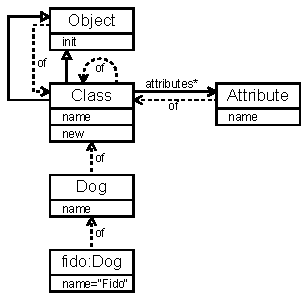
\includegraphics[width=185pt]{img/classDiagram1.pdf}
	\caption{Basic Class diagram}
	\label{fig:exampleDogClassDiagram}
\end{figure} 

Dog extends (\extends) {\ttfamily Object} .It does not extend {\ttfamily Class}. It is an instance of (\of) {\ttfamily Class}. {\ttfamily Fido} is an instance of (\of) {\ttfamily Dog}. Therefore (commonly spoken): Fido is a Dog. Dog is a Class. But: Is {\ttfamily Fido} an {\ttfamily Object}? Is {\ttfamily Dog} an {\ttfamily Object}?

Differentiate between 
\begin{itemize}
	\item the \textit{operation} of() which returns the target of the \of of-Arrow \\
and 
	\item the \textit{operator} instance? which returns true if second argument is \of of() or anything of() \of\extends inherited from
  \item isTypeOf
  \item isReallyTypeOf
\end{itemize}

\begin{figure}[ht!]
	\centering
	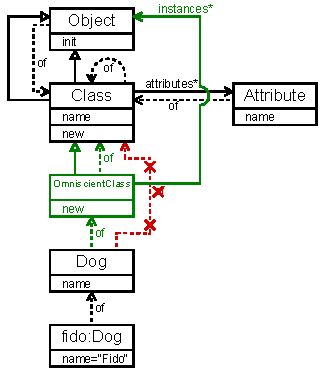
\includegraphics[width=195pt]{img/classDiagram2.pdf}
	\caption{Extended Class diagram}
	\label{fig:exampleDogClassDiagram2}
\end{figure} 

\begin{verbatim}
parserImport XOCL;

\end{verbatim}
The class {\ttfamily OmniscientClass} extends {\ttfamily Class}. Any instance of
it will therefore be a class.
\begin{verbatim}
context Root
  @Class OmniscientClass isabstract extends Class 
  @Attribute instances : Vector = Vector(12) end
  @Attribute numberInstances : Integer = 0 end
  @Attribute pluralName : String (?) end
  
  @Operation getPluralName() : String  
    name + "s"
  end
  
  @Operation new():Element
    if numberInstances >= 3 
    then let
       o = super()
       in
\end{verbatim}
This line is throwing an exception, when too many instances of the
OmniscientClass are created. It uses the function {\ttfamily getPluralName()} to
test about overwriting functions. In most cases the plural is formed by
appending a {\ttfamily s}. This is done in the default function above. The word ``Mouse''
however has an irregular plural and therefore needs to overwrite the function,
returning ``Mice'' instead of the default ``Mouses''.

Instead of overwriting functions, attributes could be used. In this case it
proves a worse choice as every slot has to be filled manually, and no useful
default can be provided.
\begin{verbatim}
          self.error("According to popular belief, " 
          + (numberInstances+1) + " " 
          + o.getPluralName() 
       // + pluralName 
          + " are deemed unlucky.")
    end
    else 
      let 
        o = super()
      in let
        c = o.of()
      in
        c.instances.put(numberInstances,o);
        self.numberInstances := numberInstances +1;
        o
      end end
    end
  end
end
\end{verbatim}
Class {\ttfamily Dog} is an instance of {\ttfamily OmniscientClass}. It is a
class because it's {\ttfamily of} is {\ttfamily Class} or a any extension
thereof.
\begin{verbatim}
context Root
  @Class Dog metaclass OmniscientClass
  @Attribute name : String = "nameless Dog" end
  @Constructor(name) ! end
  @Slot OmniscientClass::pluralName = "Dogs" end
\end{verbatim}
As {\ttfamily Dog} does not extend {\ttfamily Class}, this function is not
supposed to be called. However, it can be called by {\ttfamily(Dog())()},
naturally causing an exception to be thrown somewhere in {\ttfamily super()}.
It can be called without an exception if {\ttfamily Dog} would extend {\ttfamily Class}.
\begin{verbatim}
  @Operation new():Element
    "Dog.new".println();
    super()
  end
end

context Root
  @Class Cat metaclass OmniscientClass
  @Attribute name : String = "nameless Cat" end
  @Constructor(name) ! end
  @Slot OmniscientClass::pluralName = "Cats" end
end
\end{verbatim}
The class {\ttfamily Mouse} 
\begin{verbatim}
context Root
  @Class Mouse metaclass OmniscientClass
  @Attribute name : String = "nameless Mouse" end
  @Constructor(name) ! end
  @Slot OmniscientClass::pluralName = "Mice" end
  @Operation getPluralName() : String  
    "Mice"
  end
end

  Root::dog1 := Dog.new();
  Root::dog1.name := "Fido";
  Root::mouse1 := Mouse("Mickey");
\end{verbatim}



 Objects have a type and slots. The type is returned by the of() operation and the slots are accessed by name either using the '.' operator or the get(name) operation. Values of slots can be updated using the o.s := v notation or the o.set(s,v) operator. Messages can be sent to an object using the o.m(a1,a2,...) notation or using the o.send(m,Seq{a1,a2,...}) operator.
\vspace{3mm}

Objects implement a MOP via their meta-class that determines how slot access and update is handled. The MOP is defined on an objects type via the getInstanceSlot, hasInstanceSlot and setInstanceSlot operations. Define a new meta-class (sub-class of Class) that implements a new MOP and therefore handles object storage completely differently to the VM. 
\vspace{3mm}

\textbf{Slot storage} is usually allocated when a class is instantiated and \textbf{is always consistent with the attributes defined by the class}. You can modify this using addStructuralFeature and removeStructuralFeature, but you \textbf{must be aware that certain key execution features of XMF rely on the slots of an object conforming to the attributes of its class}. NB adding new slots to an object that do not clash with these attributes is safe and can be used to squirrel away information in particular objects.

\layerThree{Multilevel Draft Essen} 

Extend Association, Attribute, Compiled Operation by isIntrinsic, instLevel, isCore and Constraint and Doc by id.

new class/interface MetaAdapter overriding new(decreasing level by one) with additional function newAtLevel(decreasing level by more than one) 

???

Is a level $<=1$ (class, object) automatically forbidden to extend MetaAdapter/Class?
Is a level 0 (object) automatically forbidden to be of type MetaAdapter/Class?
Is an element which does not extend MetaAdapter/Class but is of type MetaAdapter/Class automatically a level 1?
Is an element which is not of type MetaAdapter/Class automatically a level 0?

Why start numbering levels at object level?
This means: a classic object is always level 0, a classic class always level 1.
Therefore it is always necessary to know before the number of the top layer.
Or do the upper layers number automatically? But then the instLevel for attributes does not give an absolute level-distance. Maybe allow relative intLevels? Or use another concept than integer numbering.

!!!

\layerThree{next Try} 

An element $e$ is level $0$, if and only if $e.of()$ is level 1.\\
$Level_0(e)\Leftrightarrow Level_1(e.of())$\\
$Level_1(e)\Rightarrow \neg e $ inheritsFrom $ Class$.\\
$Level_1(e)\Leftrightarrow Level_2(e.of()) \wedge \neg e $ inheritsFrom $ Class$.\\
$Level_n(Class) \forall n \geq 2$

\layerThree{next Try II} 

\newpage

\layerFour{numbering up} 
Elements can be numbered by their distance to an object, if that object is given. \\
Object o's Level in respect to o is 0.
Object o's of()'s Level in respect to o is 1.
Class' Level in respect to o is the number of \textit{of()}s one has to traverse,. including but not counting \textit{inherits}.
\begin{verbatim}
  int levelUp(Element a, Element b) {
      if(a == b) return 0;
      if(b.of() != b) return 1 + levelUp(a, b.of());
      if(b.inherits() != b) return levelUp(a, b.inherits());
      throw Exception;
  }
\end{verbatim}

\layerFour{numbering down} 
Elements can be numbered by their distance to \textit{Class} \\
Object o's Level in respect to \textit{Class} is the number of \textit{of()}s one has to traverse from o to Class, including but not counting \textit{inherits}. Be this number negative for easier disambiguation.
\begin{verbatim}
  int levelDown(Element e) {
      if(e == Class) return 0;
      if(e.of() != e) return -1 - levelDown(e.of());
      if(e.inherits() != e) return levelDown(e.inherits());
      throw Exception;
  } <==> {
      return - levelUp(Class, e);
  }	
\end{verbatim}

\layerFour{allowing multi-level jumps}
If we have a of-relation with a specified weight $>=1$ we can amend the formulas above nad replace 1 with the weight.
\begin{verbatim}
  int levelUp(Element a, Element b) {
      if(a == b) return 0;
      if(b.of() != b) return b.ofWeight() + levelUp(a, b.of());
      if(b.inherits() != b) return levelUp(a, b.inherits());
      throw Exception;
  }
\end{verbatim}

\newpage

\layerFour{Finding a unified numbering scheme} 

Assume the following relation:

fido \of Dog \of Quadruped \of Animal \of MetaClass \of Class

squidward \of Octopus \of Animal \of MetaClass \of Class

where (Quadruped and Animal) \extends MetaClass \extends Class

\begin{tabular}[t]{|l|l|l|l|l|l|} \hline
x&levelDown(x)&levelUp(x, fido)&levelUp(x, Octopus)&levelUp(x, Animal) \\\hline
fido 				&-5&  0& N/A&(-3) \\\hline
Dog 				&-4&  1& N/A&(-2) \\\hline
Quadruped 	&-3&  2& N/A&(-1) \\\hline
squidward 	&-4&N/A&(-1)&(-2) \\\hline
Octopus 	  &-3&N/A&   0&(-1) \\\hline
Animal 			&-2&  3&   1&   0 \\\hline
MetaClass 	&-1&  4&   2&   1 \\\hline
Class 			& 0&  5&   3&   2 \\\hline
\hline
\end{tabular}

The levelUp function can be extended downwards into negative results.

\vspace{5mm}

If we want a Slot name for every Animal, we would add an Attribute name to Animal to become a Slot on Level 0. But we cannot say which level Animal is on.\\
We cannot instantiate an animal object directly to level 0, as Animal inherits Class


%\vspace(12mm)
%Modify Existing Classes --- or add new extended classes?
\layerOne{Literature}

\begin{itemize}
  \item A Unifying Approach to Connections for Multi-Level Modeling
  \cite{article:AtkinsonGerbigKuehne2015}
  \begin{itemize}
  \item Melanie: Multi-level Modeling and Ontology Engineering
  Environment \cite{article:AtkinsonGerbig2012}
  \item Referenced 2
  \item Referenced 3
\end{itemize}
\end{itemize}

\layerTwo{Integrating Language Engineering\cite{article:ClarkFrank0000}...}




\nocite{article:test}


\begin{itemize}
\lowItem XModeler
\begin{itemize}
  \lowItem What is XModeler?
	\lowItem Getting started
	\begin{itemize}
		\lowItem Install guide
		\lowItem Tutorial
	\end{itemize}
	\lowItem Help
	\begin{itemize}
		\lowItem API
		\lowItem Language concepts
		\lowItem Snippets $^X$
		\lowItem Bluebook $^X$
	\end{itemize}
\end{itemize}
\lowItem Literature
\begin{itemize}
	\lowItem Articles, Papers
		\begin{itemize}
		\lowItem Our Articles, Papers
		\lowItem Conferences
		\lowItem List of others' literature
	\end{itemize}
	\lowItem Lecture Slides and other material for students $^O$
\end{itemize}
\lowItem External Links
\begin{itemize}
	\lowItem git
	\lowItem shu
	\lowItem ude
\end{itemize}
\lowItem Contact
\begin{itemize}
	\lowItem Who are we
	\lowItem How to contact us
	\lowItem Impressum
\end{itemize}
\end{itemize}
 $^X$: Not available online\newline
 $^O$: Only available online\newline
\newline
Is any material we use copyrighted? Are icons and logos in XModeler our work? If they are from any "`free"' source, are there any conditions on them?\newline
Do we need any legal advice? Disclaimers?
\\
\layerOne{Weekly Reports}
\setcounter{section}{14}
\layerTwo{2015}
\setcounter{subsection}{36}

\layerThree{7 Sep 2015 - 11 Sep 2015}
\begin{itemize}
\item Made browser tabs closeable
\item Init Requirements and Specifications in LaTeX
\item Added Panic button to GUI
\item Image loading: XML file now derived from IMG file name and path instead of storing
that information in the IMG file.
\item Division of BigIntegers fixed, Multiplication of negative Integers fixed
\end{itemize}

\layerThree{14 Sep 2015 - 18 Sep 2015}
\begin{itemize}
\item Tested and documented some git features.
\item Produced conflicts in git: Managed to resolve them finally. It was challenging. Further
testing required.
\item Tried to install safari. Waiting for Help desk...
\item Made the browser work again. Several fixes: Removed layouter, changed locking mechanism,
set to native browser
\end{itemize}

\layerThree{21 Sep 2015 - 25 Sep 2015}
Used XMF to do exercises with meta-classes \begin{itemize} 
\item to understand the concept of class, object, instantiation and inheritance
\item to override the default meta-object-protocol, be redefining new/get/set etc.
\item to understand the default behaviour of XMF
\end{itemize}

\layerThree{28 Sep 2015 - 2 Oct 2015}
\begin{itemize} 
\item Continued experiments with meta-classes
\item Gathered ideas for website; some experiments with html.
\end{itemize}

\layerThree{5 Oct 2015 - 9 Oct 2015}
\begin{itemize} 
\item Preparation for discussions about intrinsics.
\item Fr: Travel
\end{itemize}

\layerThree{12 Oct 2015 - 16 Oct 2015}
\begin{itemize} 
\item Mo,Tu,Fr: holiday
\item Making documentation for sceanarios for changes on intrinsic attributes
\item Tiny bugfix in FormsClient
\end{itemize}

\layerThree{19 Oct 2015 - 23 Oct 2015}
\begin{itemize} 
\item Mo: Travel
\item Added Monospace (with anti-alias) font to editor window.
\end{itemize}

\layerThree{26 Oct 2015 - 30 Oct 2015}
\begin{itemize} 
\item Started to fix HTML generation
\end{itemize}

\layerThree{2 Nov 2015 - 6 Nov 2015}
\begin{itemize} 
\item Fixed Live Documentation
\item Drew diagram for intrinsics to verify current model
\end{itemize}

\layerThree{9 Nov 2015 - 13 Nov 2015}
\begin{itemize} 
\item fix syntax highlighting
\item fix \%20 at welcome page
\end{itemize}

\layerThree{16 Nov 2015 - 20 Nov 2015}
\begin{itemize} 
\item fix fonts, test change fonts dynamically
\item fix autocomplete . , ()
\item remove debug noDocFound, isLikelyToBeHTML
\end{itemize}

\layerThree{23 Nov 2015 - 27 Nov 2015}
\begin{itemize} 
\item Diagrams: added InstLevel to associations
\item fixed zoom
\end{itemize}

\layerThree{30 Nov 2015 - 3 Dec 2015}
\begin{itemize} 
\item Modified appearance of associations, added arrows
\item Added boxes for intrinsic Level
\item Multiplicity shows always
\end{itemize}

\layerThree{9 Dec 2015 - 10 Dec 2015}
\begin{itemize} 
\item Visit in Essen
\end{itemize}

\layerThree{14 Dec 2015 - 18 Dec 2015}
\begin{itemize} 
\item Changed label's and arrow's position on associations in diagrams
\item Tried to make DEL-key work in diagrams
\end{itemize}

\layerThree{ToDo}
\begin{itemize}
\item improve webpage
\item Specify FormClient, fix only
\item git commands in Eclipse
\item (nextWeek) MeMo language requirements
\item pw protected folder: \url{https://wincent.com/wiki/git_repository_access_control}
\item Snippets
\item look at/play with Kernel (Object/Class/Attribute)
%\item Use Notepad++ with syntax highlighting for user defined languages: \url{http://weblogs.asp.net/jongalloway/creating-a-user-defined-language-in-notepad}
\item HTMLViewer.xmf: Are ".o", ".xip", ".xto", ".xtd", ".xtml" still in use?
Welcome.xmf: requestURL ...
requirements
\item welcome page does not work in linux
\item experiment: call java function
%\item fix documentation bug (over lunch)
\item rectangular edges only on some edge types
\item Show/hide in Diagram
\item show warning in diagram when drawing nonsense
\item supporting multiple languages
\end{itemize}


\clearpage
\phantomsection
\addcontentsline{toc}{chapter}{Bibliography}
\bibliography{literature}
\bibliographystyle{literatureStyle}
\end{document}
